\documentclass[11pt,a4paper]{article}

% ---------- Encoding & Language ----------
\usepackage[english]{babel}

% ---------- Fonts ----------
\renewcommand{\bfdefault}{b}
\usepackage{textcomp}
\usepackage{iftex}

\ifPDFTeX
  \usepackage[utf8]{inputenc}
  \usepackage[T1]{fontenc}
  \usepackage{lmodern}
  \usepackage[final,protrusion=true,expansion=true]{microtype}
\else
  \usepackage{fontspec}
  \usepackage[final,protrusion=true,expansion=false]{microtype}
\fi

% ---------- Bengali-script support ----------
% Renders inline Bangla glyphs when a Bengali font is available (XeLaTeX/LuaLaTeX
% with polyglossia, or pdfTeX if a Bengali package is loaded). Falls back to a
% bracketed romanisation under plain pdfTeX so the source always compiles.
\newif\ifbnavailable
\ifPDFTeX
  \IfFileExists{bangla.sty}{%
    \usepackage{bangla}\bnavailabletrue
  }{\bnavailablefalse}
\else
  \usepackage{polyglossia}
  \setmainlanguage{english}
  \IfFontExistsTF{Noto Sans Bengali}{%
    \newfontfamily\bengalifont{Noto Sans Bengali}[Script=Bengali]%
    \setotherlanguage{bengali}\bnavailabletrue
  }{\bnavailablefalse}
\fi
% \bn{<bengali>}{<roman fallback>} — prints Bengali if available, else the fallback.
\ifbnavailable
  \ifPDFTeX
    \newcommand{\bn}[2]{{\bntext #1}}
  \else
    \newcommand{\bn}[2]{{\bengalifont #1}}
  \fi
\else
  \newcommand{\bn}[2]{\emph{#2}}
\fi

% ---------- Math ----------
\usepackage{amsmath,amssymb,amsthm,mathtools}
\usepackage{bm}

% ---------- Page Layout ----------
\usepackage[a4paper,
            top=1.7cm, bottom=1.7cm,
            left=2.0cm, right=2.0cm,
            headheight=14pt, headsep=12pt, footskip=22pt]{geometry}
\renewcommand{\topfraction}{0.92}
\renewcommand{\bottomfraction}{0.7}
\renewcommand{\textfraction}{0.08}
\renewcommand{\floatpagefraction}{0.85}

\usepackage{setspace}
\setstretch{1.0}

\usepackage{parskip}
\setlength{\parskip}{0.35em plus 0.1em}

% ---------- Colour Palette ----------
\usepackage{xcolor}
\definecolor{accent}{RGB}{30,72,128}
\definecolor{accent2}{RGB}{120,30,40}
\definecolor{abstractbg}{RGB}{242,242,244}
\definecolor{abstractrule}{RGB}{200,200,206}
\definecolor{tablerow}{RGB}{246,246,249}
\definecolor{capgrey}{RGB}{60,60,60}

% ---------- Headers & Footers ----------
\usepackage{fancyhdr}
\pagestyle{fancy}
\fancyhf{}
\renewcommand{\headrulewidth}{0.4pt}
\renewcommand{\footrulewidth}{0pt}
\fancyhead[L]{\small\itshape S.\,Alam, N.\,Parvez, A.\,F.\,M.\,M.\,Rahman}
\fancyhead[R]{\small\itshape BanglaCyberBench}
\fancyfoot[C]{\thepage}

\fancypagestyle{firstpage}{%
  \fancyhf{}%
  \renewcommand{\headrulewidth}{0pt}%
  \fancyfoot[C]{\thepage}%
}

% ---------- Section Headings ----------
\usepackage[explicit]{titlesec}
\titleformat{\section}[block]
  {\large\bfseries\color{accent}\sffamily}
  {\thesection.}{0.5em}{#1}[\vspace{-0.3em}{\color{abstractrule}\rule{\linewidth}{0.4pt}}]
\titleformat{\subsection}[block]
  {\normalsize\bfseries\sffamily}
  {\thesubsection}{0.5em}{#1}
\titleformat{\subsubsection}[block]
  {\normalsize\bfseries\sffamily\itshape}
  {\thesubsubsection}{0.5em}{#1}
\titlespacing*{\section}{0pt}{1.0em}{0.4em}
\titlespacing*{\subsection}{0pt}{0.6em}{0.2em}
\titlespacing*{\subsubsection}{0pt}{0.7em}{0.2em}

% ---------- Graphics & Tables ----------
\usepackage{graphicx}
\graphicspath{{figures/}}
\usepackage{booktabs}
\usepackage{multirow}
\usepackage{makecell}
\usepackage{array}
\usepackage{tabularx}
\usepackage{colortbl}
\arrayrulecolor{black!75}
\renewcommand{\arraystretch}{1.0}
\usepackage{caption}
\captionsetup{font={small,color=capgrey},labelfont={bf,color=accent},
              labelsep=period,skip=3pt,
              justification=justified,singlelinecheck=false}
\usepackage{subcaption}
\usepackage{float}

% ---------- Algorithms ----------
\usepackage{algorithm}
\usepackage{algpseudocode}

% ---------- Hyperlinks & Citations ----------
\usepackage[colorlinks=true,
            linkcolor=accent,
            citecolor=accent,
            urlcolor=accent,
            filecolor=accent,
            bookmarksopen=true]{hyperref}
\usepackage[noabbrev,capitalise]{cleveref}

\pdfstringdefDisableCommands{%
  \def\dset#1{#1}%
  \def\citet#1{[#1]}%
  \def\citep#1{[#1]}%
  \def\Cref#1{Section}%
  \def\cref#1{section}%
  \def\texttt#1{#1}%
  \def\textsc#1{#1}%
  \def\emph#1{#1}%
  \def\bfseries{}%
  \def\sffamily{}%
  \def\itshape{}%
}

\usepackage[numbers,square,sort&compress]{natbib}
\bibliographystyle{IEEEtranN}
\setlength{\bibsep}{1pt plus 0.5pt}

% ---------- Misc ----------
\usepackage{enumitem}
\setlist{itemsep=2pt,topsep=3pt,parsep=0pt}
\usepackage{url}
\usepackage{ragged2e}

% ---------- Abstract Box ----------
\usepackage[most]{tcolorbox}
\newtcolorbox{journalabstract}{
  enhanced,
  colback=abstractbg,
  colframe=abstractrule,
  boxrule=0.4pt,
  arc=2pt,
  left=10pt,right=10pt,top=7pt,bottom=7pt,
  fontupper=\small,
  before skip=8pt,after skip=8pt,
}

% ---------- Footnote tweaks ----------
\renewcommand{\footnoterule}{\noindent\rule{0.4\linewidth}{0.4pt}\vspace{2pt}}

% ---------- Convenience commands ----------
\providecommand{\dset}[1]{\textsc{#1}}
\newcommand{\bench}{\textsc{BanglaCyberBench}}

% =============================================================
\begin{document}

\thispagestyle{firstpage}

\vspace{0.5em}
% --- Title ---
{\RaggedRight\sffamily\bfseries\Large\color{black}%
\bench{}: A Dual-Script Benchmark and a Script-Aware\\[1pt]
Ensemble for Bengali Cyberbullying Detection\par}
\vspace{0.6em}

% --- Authors ---
{Sefayet Alam\textsuperscript{1,$\ast$},\quad
Naim Parvez\textsuperscript{1},\quad
A.\,F.\,M.~Minhazur Rahman\textsuperscript{1}\par}
\vspace{0.3em}

% --- Affiliation ---
{\textsuperscript{1}Department of Computer Science and Engineering,
Rajshahi University of Engineering \& Technology (RUET), Rajshahi-6204, Bangladesh\par}
\vspace{0.2em}

{\small\textsuperscript{$\ast$}\textbf{Corresponding author:} Sefayet Alam;
\href{mailto:sefayetalam14@gmail.com}{\texttt{sefayetalam14@gmail.com}}\par}

\vspace{0.5em}
{\color{abstractrule}\rule{\linewidth}{0.4pt}}
\vspace{0.3em}

% =============================================================
% ABSTRACT
% =============================================================
\begin{journalabstract}
\noindent\textbf{Abstract.\;}%
Bengali cyberbullying detection has been studied almost entirely on single sources, in a single script (Bangla), with coarse labels, and without any test of how models behave under distribution shift. That leaves open the question a deployed moderation system actually faces: will a classifier trained on one collection still work on comments it has never seen, written in a script it was not built for? We take up that question with two things. The first is \bench{}, a deduplicated four-source benchmark of \textbf{94{,}323} unique comments spanning Bangla script and Romanized Bangla (\emph{Banglish}), consolidated from 135{,}575 raw rows into a clean five-class taxonomy (\emph{none, abusive, sexual, religious, threat}) through a documented priority rule over 89 raw label strings. The second is a script-aware ensemble: four encoders (BanglishBERT, a Bangla-script-specialist BanglaBERT that is masked off Romanized rows, MuRIL, and XLM-R), each fine-tuned with a deliberately minimal recipe of cross-entropy plus Fast Gradient Method (FGM) adversarial training, fused by a validation-optimised weighted-logit rule. The minimalism is not a guess; a component ablation shows that of the usual imbalance and regularisation tricks, only a few help and one (a balanced sampler) hurts, so the proposed model keeps FGM and drops the rest. On the official 20\% test split the ensemble reaches Macro-F1 \textbf{0.8225} (95\% bootstrap CI $[0.8151, 0.8298]$), Weighted-F1 0.8332, Accuracy 0.8339, MCC 0.7452, and Macro-AUROC 0.9626, comfortably above the strongest non-transformer reference. Held one source out at a time, Macro-F1 falls to 0.46--0.60, which quantifies how much in-domain accuracy overstates cross-source readiness. On the base paper's own Facebook-44K, five-class protocol the proposed model reaches Macro-F1 0.8679 with four backbones against the base paper's 0.8923 with three, while improving the hardest class, \emph{Threat}, by more than seven F1 points (0.8292 vs.\ 0.7579). The benchmark, splits, and code are released.

\vspace{4pt}
\noindent\textbf{Keywords:}\; Bengali cyberbullying detection;\; Romanized Bangla;\; dual-script benchmark;\; script-aware ensemble;\; adversarial fine-tuning;\; class imbalance;\; cross-source robustness.
\end{journalabstract}

\vspace{0.2em}

% =============================================================
% SECTION 1 — INTRODUCTION
% =============================================================
\section{Introduction}
\label{sec:introduction}

Cyberbullying on social platforms is a daily reality for a large share of Bengali-speaking users, and the volume of it makes manual moderation hopeless. Bengali is spoken by more than 240 million people, yet it sits on the low-resource side of NLP: annotated corpora are small, they come from scattered sources with incompatible label schemes, and a large fraction of real abusive text is not even written in Bangla script. People routinely type Bengali in the Latin alphabet, so \emph{tui akta faltu manush} and its Bangla-script equivalent carry the same insult in two different surface forms. A moderation model that only ever saw one of those forms is blind to the other, and most published Bengali cyberbullying work has looked at exactly one of them.

Three limitations run through the prior literature. Datasets are almost always single-source, so a model learns one platform's quirks and one annotation team's habits rather than the phenomenon itself. The script is almost always Bangla-only, so Romanized Bangla, which is ubiquitous in comments, is left untested. And evaluation almost always stops at a random split of the one corpus, so nothing tells us whether the model transfers. The strongest recent system, the transformer-stacking framework of \citet{hoque2025transformerstacking}, reports 89.23\% multiclass F1 on a 44{,}001-comment Facebook dataset, which is a genuinely strong single-source number, but it is a single-source number: one platform, one script, and no measurement of what happens off that distribution.

This paper is built around the gap those three limitations leave. We ask whether heterogeneous Bengali cyberbullying data can be unified into one clean, deduplicated, dual-script, fine-grained benchmark; whether a compact, script-aware model can classify abuse across both scripts without the heavy regularisation stack that is usually thrown at imbalanced text; and how far such a model actually travels when a whole source or a whole script is held out. We answer all three, and we are deliberate about separating what is solved (in-domain, fine-grained classification) from what is not (cross-source and, especially, cross-script transfer).

\subsection{Contributions}
\label{sec:contributions}

\textbf{(C1) A multi-source, dual-script, deduplicated benchmark.} \bench{} merges four public Bengali datasets into 94{,}323 unique comments after removing 41{,}252 duplicate rows, covering Bangla script (60.4\%) and Romanized Bangla (39.6\%) under one schema. A hard \texttt{uid} intersection assertion guarantees no comment leaks across splits.

\textbf{(C2) A documented five-class taxonomy.} Eighty-nine raw label strings from four incompatible schemas are folded into five semantically coherent classes by an explicit priority rule, keeping explicit-violence and identity-targeted abuse from being swallowed by a generic bucket.

\textbf{(C3) A script-aware ensemble with a minimal, ablation-justified recipe.} Four encoders are fine-tuned with cross-entropy plus FGM only; a component ablation on the real imbalanced data drives that minimalism, and a Bangla-only specialist is masked off Romanized rows in the fusion.

\textbf{(C4) A cross-source robustness study.} We hold each source out in turn and measure the drop, giving the first source-transfer picture for this task and showing that in-domain accuracy badly overstates deployment readiness.

\textbf{(C5) A same-protocol comparison against the base paper.} On the base paper's own Facebook-44K five-class split we retrain the proposed model and report a like-for-like comparison, competitive overall with a clear gain on the rare \emph{Threat} class.

\textbf{(C6) Statistically grounded reporting and an open release.} Headline and per-class numbers carry bootstrap 95\% confidence intervals; the benchmark, splits, and code are released.

The rest of the paper is organised as follows. \Cref{sec:related-work} reviews prior work; \cref{sec:benchmark} describes the benchmark and its construction; \cref{sec:methodology} formalises the proposed model on a single comment; \cref{sec:setup} gives the experimental setup; \cref{sec:results} reports results; \cref{sec:discussion} discusses them; and \cref{sec:conclusion} concludes.

% =============================================================
% SECTION 2 — RELATED WORK
% =============================================================
\section{Related Work}
\label{sec:related-work}

\subsection{Bengali Cyberbullying and Hate-Speech Detection}
\label{sec:rw-bengali}

Early Bengali abuse detection leaned on classical machine learning over surface features. TF-IDF with logistic regression, SVMs, and tree ensembles was the standard toolkit \citep{ahmed2021deployment,akhter2023robust,saha2023bengali}, and it works until the abuse stops being lexical. \citet{akhter2023robust} pushed a hybrid machine-learning model for Bengali cyberbullying but stayed with a single Bangla-script source. Deep learning shifted the ceiling: BiLSTM and CNN-BiLSTM models with FastText or GloVe embeddings \citep{romim2021hateban,nath2024deeplearning} captured more context, though they too kept to single corpora. The move to transformers is recent and clear. \citet{emon2022detection} and \citet{aurpa2022abusive} applied BERT-family encoders to Bangla abusive-comment detection; \citet{karim2021deephateexplainer} added explainability to Bengali hate-speech classification; and \citet{saifullah2024cyberbullying} combined deep learning with transformer language models. The base paper for this study, \citet{hoque2025transformerstacking}, stacks XLM-R, mBERT, and Bangla-BERT-Base under an MLP meta-classifier and reaches strong numbers on a 44{,}001-comment Facebook corpus. It is the current high-water mark on that dataset, and it is also the clearest example of the single-source, single-script, no-shift pattern this paper pushes against.

Datasets have grown alongside the methods. \citet{romim2021hate} released a Bengali hate-speech corpus with baseline evaluation; \citet{ahmed2021bangla} built a Facebook harassment dataset with exploratory analysis; regional and multi-task resources such as \dset{BIDWESH} \citep{gomes2025bidwesh} and LLM-based multi-task hate-speech corpora \citep{banglamultihate2025} broadened coverage into dialects and severity. What is still missing is a single benchmark that unifies several of these sources, removes the duplicate leakage that quietly inflates accuracy, and covers both scripts at once. \Cref{tab:priordata} places \bench{} against representative prior resources on the axes that matter for this paper: number of sources, script coverage, taxonomy granularity, and whether cross-distribution transfer was ever measured. \bench{} is designed around the empty column, dual-script coverage tested under held-out shift.

\begin{table}[!htbp]
\centering
\caption{Representative Bengali abuse-detection resources against \bench{}. ``Shift tested'' asks whether the study measured transfer to an unseen source or script rather than only a random in-domain split.}
\label{tab:priordata}
\small
\begin{tabularx}{\textwidth}{@{}lcccc>{\raggedright\arraybackslash}X@{}}
\toprule
\textbf{Resource} & \textbf{Sources} & \textbf{Script} & \textbf{Classes} & \textbf{Shift tested} & \textbf{Size} \\
\midrule
Romim et al.\ \citep{romim2021hate} & 1 & Bangla & binary & no & 30k \\
Ahmed et al.\ \citep{ahmed2021deployment} & 1 & Bangla + Rom. & binary & no & 10k \\
Karim et al.\ \citep{karim2021deephateexplainer} & 1 & Bangla & multi & no & 8k \\
Base paper \citep{hoque2025transformerstacking} & 1 & Bangla & 5 & no & 44k \\
\textbf{\bench{} (ours)} & \textbf{4} & \textbf{Bangla + Rom.} & \textbf{5} & \textbf{yes} & \textbf{94k} \\
\bottomrule
\end{tabularx}
\end{table}

\subsection{Romanized Bangla and the Script Problem}
\label{sec:rw-script}

Romanized Bangla is not a niche. A large fraction of Bengali social-media text is typed in the Latin alphabet, with no spelling standard, heavy code-mixing with English, and free vowel-dropping. \citet{ahmed2021deployment} is one of the few studies to treat Bangla and Romanized Bangla side by side, and it does so with classical models on a modest scale. The pretrained-encoder landscape reflects the split: BanglaBERT \citep{bhattacharjee2022banglabert} is an ELECTRA-style discriminator pretrained on 27.5\,GB of Bangla-script text and is state of the art on Bangla-script understanding, while its sibling BanglishBERT is pretrained bilingually on Bangla and English and is the natural choice for Romanized input. MuRIL \citep{khanuja2021muril} adds transliterated Indian-language text, and XLM-R \citep{conneau2020xlmr} is a broad multilingual baseline. A recurring, under-tested assumption is that one encoder can serve both scripts. Our robustness results question that assumption directly, and the script-aware design in \cref{sec:methodology} is our response to it.

\subsection{Adversarial and Imbalance-Aware Fine-Tuning}
\label{sec:rw-methods}

Perturbing continuous word embeddings during training is a cheap, reliable regulariser for small-data text classification. The Fast Gradient Method \citep{miyato2017adversarial}, a text adaptation of the image-domain idea of \citet{goodfellow2015explaining}, adds one adversarial forward-backward pass per batch and consistently steadies fine-tuning. Complementary tricks target class imbalance and overfitting: focal loss \citep{lin2017focal} and class-balanced weighting \citep{cui2019classbalanced} down-weight easy majority examples, multi-sample dropout \citep{inoue2019multisample} reduces head variance, R-Drop \citep{liang2021rdrop} enforces consistency between two dropout passes, weight averaging in the style of mean teachers \citep{tarvainen2017meanteacher} stabilises evaluation weights, and logit adjustment \citep{menon2021longtail} corrects the long tail at inference. The usual instinct is to stack all of them. Our ablation (\cref{sec:ablation-results}) shows that instinct is wrong on this benchmark: several of these add little, one hurts, and the full stack underperforms a lean cross-entropy-plus-FGM recipe. That finding is what makes the proposed model minimal by design rather than by omission.


% =============================================================
% SECTION 3 — BENCHMARK
% =============================================================
\section{The \bench{} Benchmark}
\label{sec:benchmark}

\bench{} merges four public Bengali datasets into one deduplicated, dual-script, five-class corpus. \Cref{fig:pipeline} shows the construction pipeline end to end; this section walks through each stage and the decisions behind it.

\begin{figure}[!htbp]
\centering
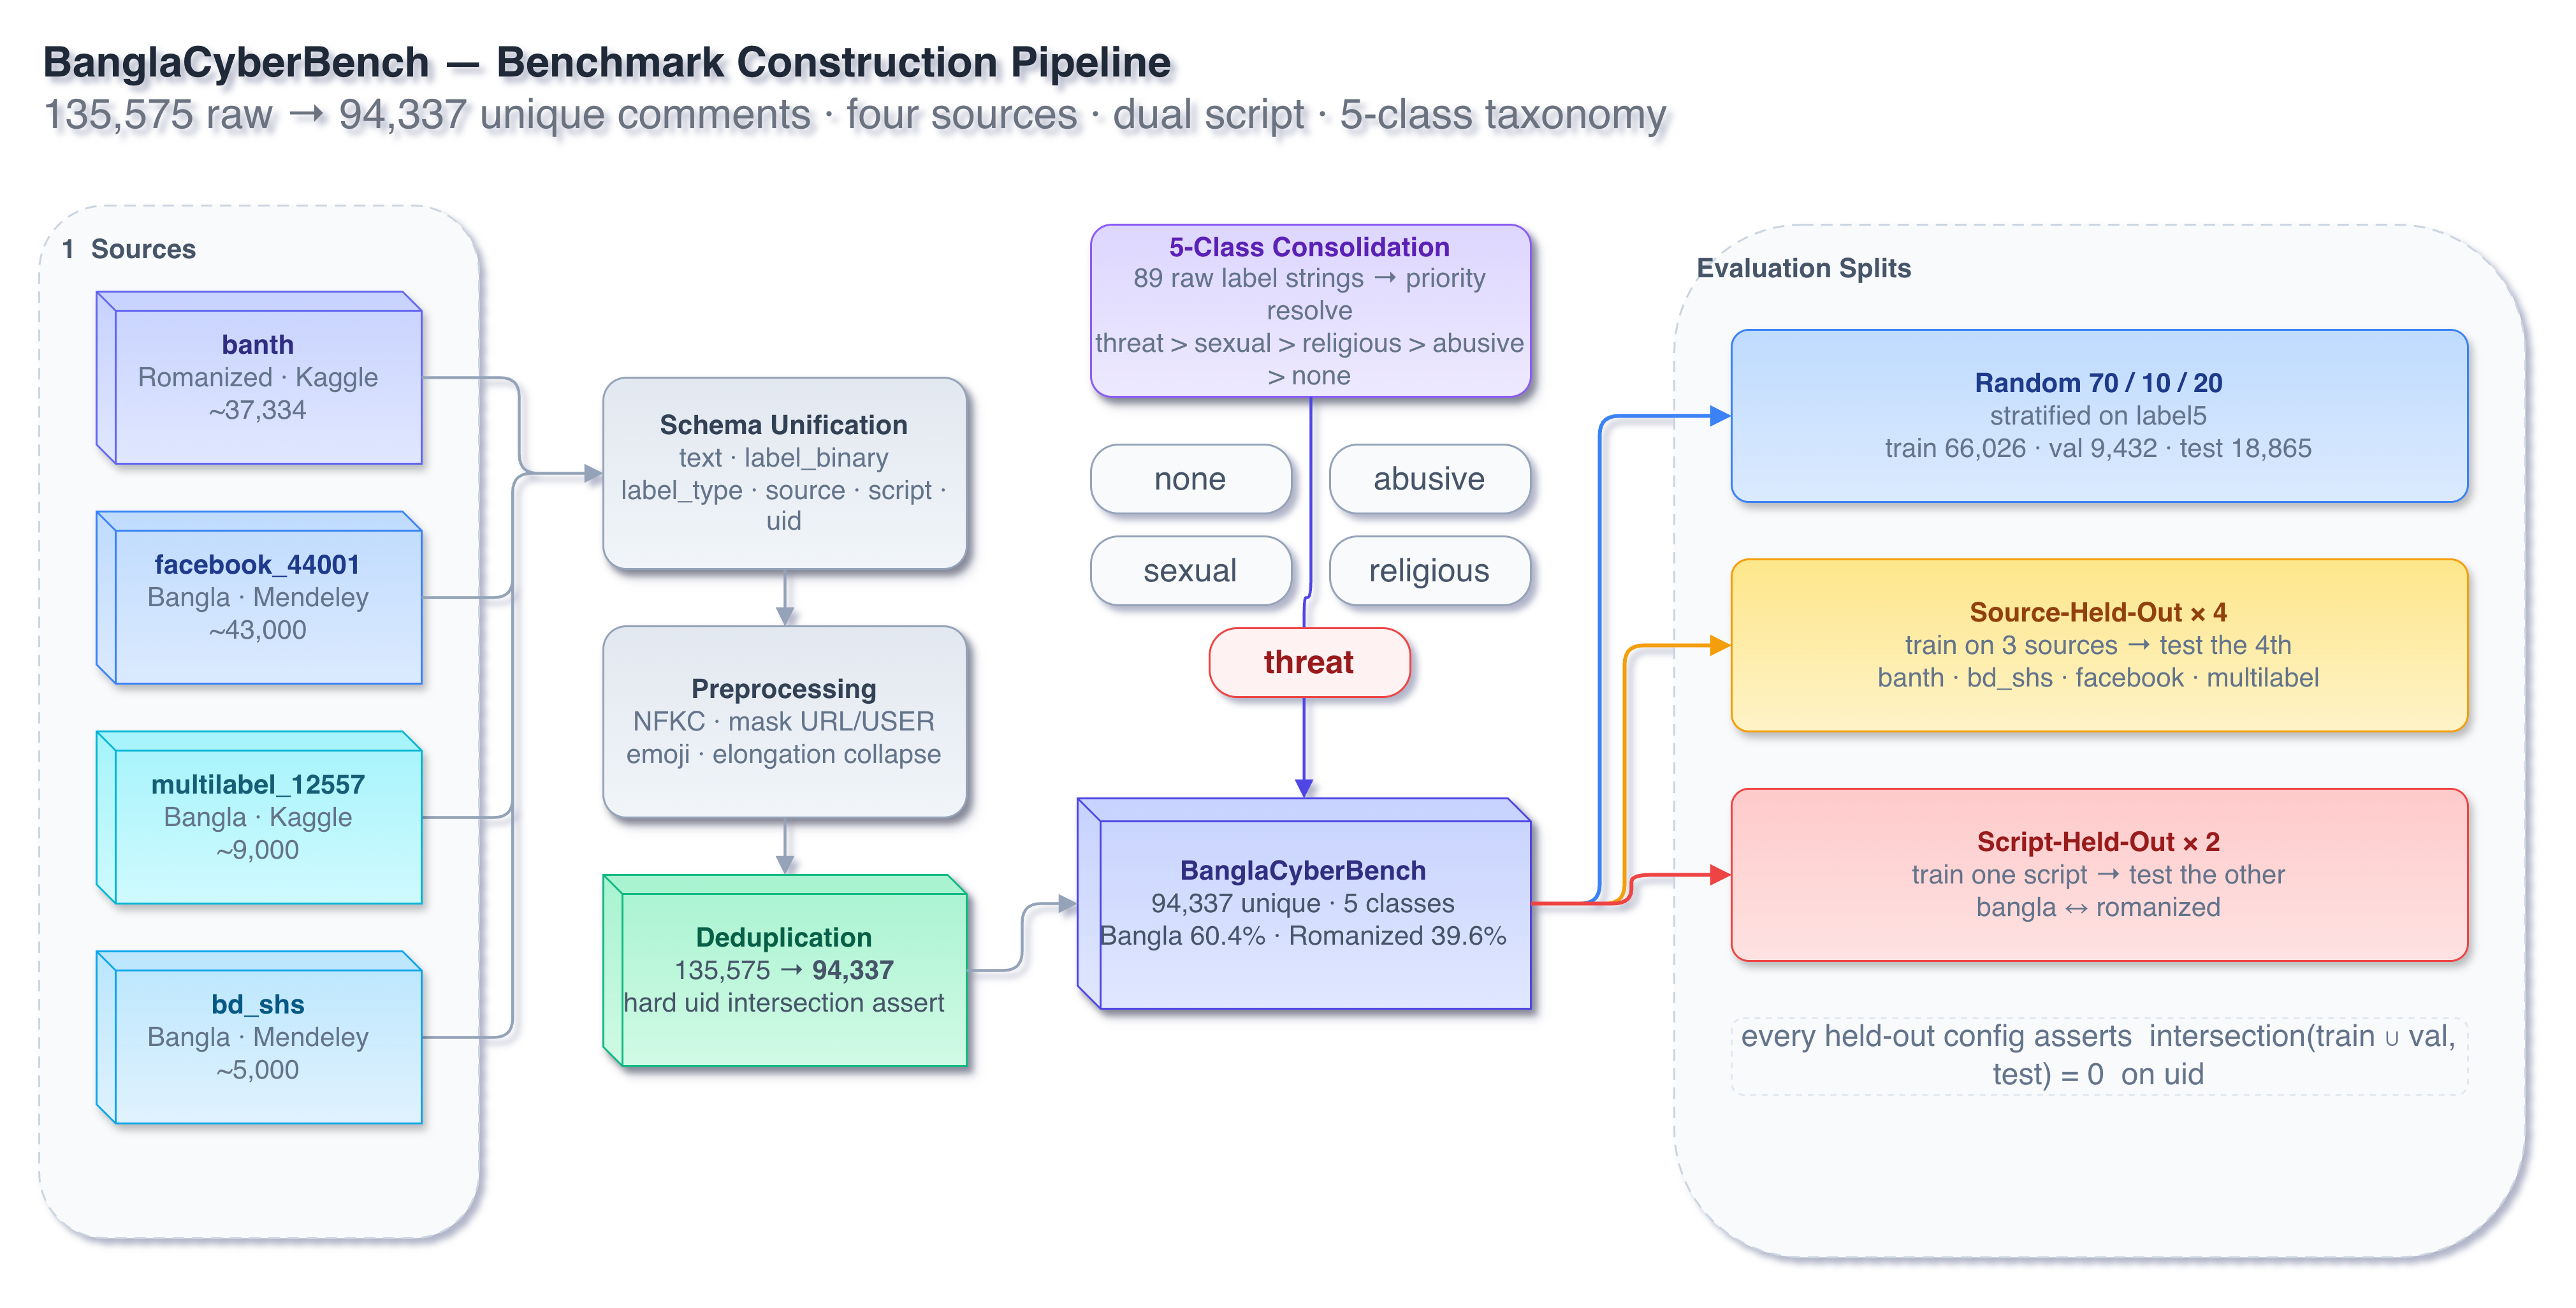
\includegraphics[width=0.98\textwidth]{D1_Benchmark_Construction.png}
\caption{Benchmark construction pipeline. Four sources are unified into a common schema, lightly normalised, deduplicated on cleaned text ($135{,}575 \rightarrow 94{,}323$), consolidated from 89 raw label strings into five classes by a priority rule, and split into a stratified random 70/10/20 partition plus source-held-out configurations. Every held-out configuration asserts a zero \texttt{uid} intersection between training and test.}
\label{fig:pipeline}
\end{figure}

\subsection{Sources and Schema Unification}
\label{sec:sources}

The four sources differ in platform, script, and label format (\cref{tab:sources}). \dset{banth} is Romanized Bangla with a binary column plus per-type indicator columns; \dset{facebook\_44001} is Bangla script with a single label column and is the base paper's source; \dset{multilabel\_12557} is Bangla with separate indicator columns; and \dset{bd\_shs} is Bangla with one harmful-flag column and one type column. We rewrite all four into a common schema, \texttt{text $\cdot$ text\_clean $\cdot$ label\_binary $\cdot$ label\_type $\cdot$ label5 $\cdot$ source $\cdot$ script $\cdot$ uid}, so that everything downstream reads one format. \dset{banth} is the only Romanized source, which is why, later, source-held-out on \dset{banth} and any cross-script analysis are closely related rather than independent.

\begin{table}[!htbp]
\centering
\caption{The four sources after deduplication. \dset{banth} is the sole Romanized-Bangla source; the other three are Bangla script. Shares are of the 94{,}323-comment benchmark.}
\label{tab:sources}
\small
\begin{tabularx}{\textwidth}{@{}lllrX@{}}
\toprule
\textbf{Source} & \textbf{Script} & \textbf{Origin} & \textbf{Samples} & \textbf{Raw label style} \\
\midrule
\dset{facebook\_44001} & Bangla & Mendeley & 43{,}078 & single label column \\
\dset{banth} & Romanized & Kaggle & 37{,}334 & binary column + 0/1 type columns \\
\dset{multilabel\_12557} & Bangla & Kaggle & 8{,}882 & separate 0/1 type columns \\
\dset{bd\_shs} & Bangla & Mendeley & 5{,}029 & one harmful column + one type column \\
\midrule
\textbf{Total} & --- & --- & \textbf{94{,}323} & --- \\
\bottomrule
\end{tabularx}
\end{table}

\subsection{Preprocessing}
\label{sec:preprocessing}

Bengali abuse leans on cues that aggressive normalisation destroys, so the cleaning is light and script-safe. We apply NFKC Unicode normalisation, strip zero-width and invisible characters, mask URLs and mentions to \texttt{[URL]} and \texttt{[USER]}, rewrite hashtags to \texttt{[HASHTAG]} while keeping the tag word, demojise emojis to bracketed text tokens, collapse runs of three or more identical characters down to two (so \emph{baaaaje} and \emph{baje} are not treated as unrelated), and normalise whitespace into \texttt{text\_clean}. We deliberately do not lowercase-fold beyond Unicode rules, strip punctuation, or remove stopwords: emphatic repetition, punctuation, and emoji all carry abuse signal, and modern subword tokenisers handle the raw form well. \Cref{fig:composition} shows the composition of the resulting benchmark by source, script, and class.

\begin{figure}[!htbp]
\centering

\includegraphics[width=0.98\textwidth]{fig_dataset_composition_pies.png}
\caption{Composition of \bench{} after deduplication ($n = 94{,}323$). Left: the four merged sources. Middle: the near-even split between Bangla script (60.4\%) and Romanized Bangla (39.6\%). Right: the five-class taxonomy, dominated by \emph{none} and \emph{abusive} with a long tail down to \emph{threat} at 3.4\%.}
\label{fig:composition}
\end{figure}

\subsection{Deduplication}
\label{sec:dedup}

Deduplication happens on \texttt{text\_clean} and before any split is drawn. The merged corpus of 135{,}575 rows collapses to 94{,}323 unique comments, removing 41{,}252 duplicates. \dset{banth} shrank the most because it carried many near-identical scrapes, which is why its post-deduplication share is smaller than its raw size would suggest. This step is not cosmetic. Undocumented duplicates are a quiet way to leak comments across splits and inflate both in-domain and held-out numbers, so a hard \texttt{uid} intersection assertion runs after every split to guarantee no comment appears in more than one partition.

\subsection{The Five-Class Taxonomy}
\label{sec:taxonomy}

The four sources together use 89 distinct raw label strings, many of them comma- or underscore-compounded (a single comment might be tagged \texttt{sexual\_threat} or \texttt{religious,abusive}). We split each raw string on \texttt{,} and \texttt{\_}, map each piece to a bucket, and resolve compounds by a fixed priority:
\begin{equation}
\textbf{threat} \;>\; \textbf{sexual} \;>\; \textbf{religious} \;>\; \textbf{abusive} \;>\; \textbf{none}.
\label{eq:priority}
\end{equation}
The order is deliberate. Explicit violence (\emph{threat}) and identity-targeted abuse (\emph{sexual}, \emph{religious}) are the classes a moderator most needs surfaced, so they win over the generic \emph{abusive} bucket when a comment carries several tags; \emph{none} loses to everything. Consistency with the binary flag is enforced: a comment flagged non-abusive resolves to \emph{none}, and one flagged abusive but resolving to \emph{none} is placed in \emph{abusive}. The resulting distribution (\cref{tab:classes}) is realistically imbalanced, with \emph{none} at half the data and \emph{threat} at 3.4\%, a roughly 14.8:1 gap between the most and least frequent class. That imbalance is the core difficulty: Macro-F1 weights every class equally, so a model that leans on the majority class is punished exactly where moderation matters most.

\begin{table}[!htbp]
\centering
\caption{Class distribution of the five-class benchmark after deduplication ($n = 94{,}323$). Raw labels folded into each class are listed in the text.}
\label{tab:classes}
\small
\begin{tabular}{@{}lrr@{}}
\toprule
\textbf{Class} & \textbf{Samples} & \textbf{Share (\%)} \\
\midrule
None & 47{,}312 & 50.16 \\
Abusive & 24{,}963 & 26.47 \\
Sexual & 10{,}822 & 11.47 \\
Religious & 8{,}032 & 8.52 \\
Threat & 3{,}194 & 3.39 \\
\midrule
\textbf{Total} & \textbf{94{,}323} & \textbf{100.00} \\
\bottomrule
\end{tabular}
\end{table}

The buckets are as follows. \emph{None} folds in \texttt{none} and \texttt{not-bully}. \emph{Abusive} is the catch-all for general offence: abusive/violence, troll, personal offence, body-shaming, origin-based slurs, slander, spam, political abuse, and miscellaneous. \emph{Sexual} folds sexual harassment and gender-based (misogynistic) harassment. \emph{Religious} folds religious and religion-directed abuse. \emph{Threat} folds explicit threats and calls to violence. \Cref{tab:consolidation} lists the full raw-string-to-bucket map used by the consolidation rule. Two consistency rules run alongside it: a component that no rule recognises but that sits under a comment flagged abusive is sent to \emph{abusive} rather than dropped, and the binary flag has the final say, so a comment flagged non-abusive resolves to \emph{none} and one flagged abusive but resolving to \emph{none} is moved to \emph{abusive}. A nine-class variant that splits the catch-all further (adding \texttt{personal, political, gender, other}) is built only for the taxonomy ablation in \cref{sec:ablation-results}, never for the headline, because those extra classes are too sparse to learn.

\begin{table}[!htbp]
\centering
\caption{Raw-label consolidation map. Each raw label string is lowercased and split on \texttt{,} and \texttt{\_}; every component is sent to a bucket, and compounds are resolved by the priority order in \cref{eq:priority}.}
\label{tab:consolidation}
\small
\begin{tabularx}{\textwidth}{@{}lX@{}}
\toprule
\textbf{Consolidated class} & \textbf{Raw components folded in} \\
\midrule
None & \texttt{none}, \texttt{not bully}, \texttt{notbully} \\
Abusive & \texttt{abusive}, \texttt{abusive/violence}, \texttt{violence}, \texttt{troll}, \texttt{personal}, \texttt{personal offense}, \texttt{political}, \texttt{slander}, \texttt{spam}, \texttt{origin}, \texttt{body shaming}, \texttt{misc} \\
Sexual & \texttt{sexual}, \texttt{gender} \\
Religious & \texttt{religious}, \texttt{religion} \\
Threat & \texttt{threat}, \texttt{calltoviolence} \\
\bottomrule
\end{tabularx}
\end{table}

\subsection{Splits and Evaluation Protocol}
\label{sec:splits}

The main split is a stratified random 70/10/20 partition on \texttt{label5}: 66{,}026 train, 9{,}432 validation, 18{,}865 test (\cref{tab:split}). Stratification holds the five-class proportions fixed across all three partitions, so the rare \emph{threat} and \emph{religious} classes keep the same share in train, validation, and test rather than drifting by chance. Validation is used only for early stopping, ensemble-weight optimisation, and any inference-time tuning; the 20\% test set is never touched during tuning, so every reported test number is a clean held-out measurement. On top of this we build four \emph{source-held-out} configurations, each testing on one unseen source while the remaining three sources are split into training and validation by a stratified 87.5/12.5 partition on \texttt{label5}; the held-out source contributes its full set of comments as the test set. This is the closest thing to a real deployment shift. Every held-out configuration re-runs the \texttt{uid} intersection assertion, so cross-split leakage is impossible by construction.

\begin{table}[!htbp]
\centering
\caption{Stratified random 70/10/20 split of the benchmark. Stratification is on the five-class label.}
\label{tab:split}
\small
\begin{tabular}{@{}lrr@{}}
\toprule
\textbf{Split} & \textbf{Samples} & \textbf{Share (\%)} \\
\midrule
Train & 66{,}026 & 70.00 \\
Validation & 9{,}432 & 10.00 \\
Test & 18{,}865 & 20.00 \\
\bottomrule
\end{tabular}
\end{table}


% =============================================================
% SECTION 4 — METHODOLOGY
% =============================================================
\section{Proposed Model}
\label{sec:methodology}

The proposed model is a script-aware ensemble of four fine-tuned transformer encoders, fused by a validation-optimised weighted-logit rule. This section traces the whole path a single comment takes through the system: tokenisation and embedding (\cref{sec:prelim}), the encoder and classification head (\cref{sec:head}), the training objective, cross-entropy plus FGM (\cref{sec:objective}), the script-aware masking that makes the ensemble aware of which alphabet a comment is written in (\cref{sec:scriptaware}), and the weighted-logit fusion that produces the final label (\cref{sec:fusion}). \Cref{fig:ensemble} shows the assembled system. \Cref{tab:notation} fixes notation.

\begin{figure}[!htbp]
\centering

\includegraphics[width=0.82\textwidth]{D2_Script_Aware_Ensemble.png}
\caption{The proposed script-aware ensemble. A comment is routed by script. All four encoders process Bangla-script comments; on Romanized comments the Bangla-script specialist BanglaBERT emits neutral logits and receives zero fusion weight, so the remaining encoders decide the label. Each encoder is fine-tuned with cross-entropy plus FGM across three seeds, and the twelve resulting logit vectors are fused by validation-optimised weights.}
\label{fig:ensemble}
\end{figure}

\begin{table}[!htbp]
\centering
\caption{Notation used in \cref{sec:methodology}.}
\label{tab:notation}
\small
\begin{tabularx}{\textwidth}{@{}lX@{}}
\toprule
\textbf{Symbol} & \textbf{Meaning} \\
\midrule
$x$, $y$ & Input comment (token sequence) and its ground-truth class \\
$T$, $C$ & Sequence length ($\le 128$ tokens) and number of classes ($C = 5$) \\
$s(x) \in \{\textsc{bn}, \textsc{rom}\}$ & Script of comment $x$: Bangla or Romanized \\
$\mathbf{e} \in \mathbb{R}^{T \times d}$ & Input-embedding matrix (token $+$ position), $d = 768$ \\
$\theta_m$, $\phi_m$ & Encoder and head parameters of backbone $m$ \\
$\mathbf{h}_t \in \mathbb{R}^{d}$ & Contextual hidden state at position $t$; $\mathbf{h}_{[\mathrm{CLS}]} \equiv \mathbf{h}_0$ \\
$\mathbf{z}_m \in \mathbb{R}^{C}$ & Logit vector from backbone $m$ \\
$\hat{p}(y \mid x) \in \Delta^{C-1}$ & Predicted class-probability vector \\
$\mathbf{r}$ & Embedding-space adversarial perturbation (FGM) \\
$\epsilon$ & FGM perturbation budget \\
$w_m \ge 0$ & Fusion weight of ensemble member $m$, $\sum_m w_m = 1$ \\
$\mathcal{M}$, $\mathcal{M}(x)$ & Full member set (12) and the active members for comment $x$ \\
\bottomrule
\end{tabularx}
\end{table}

\subsection{From a Comment to Contextual Embeddings}
\label{sec:prelim}

Take a single Romanized comment, $x = $ \emph{``tui akta faltu manush''} (roughly, \emph{``you are a worthless person''}). A backbone's subword tokeniser turns it into a sequence of $T$ token ids with a leading \texttt{[CLS]} and trailing \texttt{[SEP]}, and an embedding layer maps those ids, together with position indices, to the matrix $\mathbf{e} \in \mathbb{R}^{T \times d}$. The encoder is a stack of $L = 12$ transformer blocks \citep{vaswani2017attention}. Each block refines a sequence $\mathbf{H} \in \mathbb{R}^{T \times d}$ through self-attention,
\begin{equation}
\mathbf{Q} = \mathbf{H}\mathbf{W}^Q, \quad \mathbf{K} = \mathbf{H}\mathbf{W}^K, \quad \mathbf{V} = \mathbf{H}\mathbf{W}^V,
\qquad
\mathrm{Attn}(\mathbf{Q},\mathbf{K},\mathbf{V}) = \mathrm{softmax}\!\left(\frac{\mathbf{Q}\mathbf{K}^{\top}}{\sqrt{d_k}}\right)\mathbf{V},
\label{eq:attention}
\end{equation}
run in $H$ parallel heads and concatenated, $\mathrm{MHA}(\mathbf{H}) = \mathrm{Concat}(\mathrm{head}_1,\ldots,\mathrm{head}_H)\mathbf{W}^O$, then followed by a position-wise feed-forward network and residual-plus-LayerNorm wrappings,
\begin{equation}
\mathbf{H}' = \mathrm{LN}\!\big(\mathbf{H} + \mathrm{MHA}(\mathbf{H})\big),
\qquad
\mathbf{H}'' = \mathrm{LN}\!\big(\mathbf{H}' + \mathrm{FFN}(\mathbf{H}')\big).
\label{eq:block}
\end{equation}
Self-attention is what lets the model tie \emph{faltu} (``worthless'') to \emph{manush} (``person'') even though the insult lives in their combination, not either word alone. Stacking the twelve blocks on top of $\mathbf{e}$ yields contextual hidden states $(\mathbf{h}_0, \ldots, \mathbf{h}_{T-1})$.

Two of our backbones, BanglaBERT and BanglishBERT \citep{bhattacharjee2022banglabert}, are pretrained as ELECTRA discriminators \citep{clark2020electra} rather than masked language models: a small generator replaces some tokens and the discriminator learns to flag which ones were replaced, an objective that yields strong Bengali representations from 27.5\,GB of text. MuRIL and XLM-R are standard masked-LM encoders. For our purposes the pretraining objective matters only through the representations it produces; the fine-tuning path below is identical across all four.

\subsection{Pooling and Classification Head}
\label{sec:head}

Each backbone $m$ carries the same lightweight head. We pool the sequence by blending the \texttt{[CLS]} vector with a mean over token states, which is steadier than \texttt{[CLS]} alone on short, noisy comments:
\begin{equation}
\mathbf{h}_{\mathrm{pool}} = \tfrac{1}{2}\,\mathbf{h}_{[\mathrm{CLS}]} + \tfrac{1}{2}\cdot\frac{\sum_{t=1}^{T} m_t\,\mathbf{h}_t}{\sum_{t=1}^{T} m_t},
\label{eq:pool}
\end{equation}
where $m_t \in \{0,1\}$ is the attention mask that zeroes out padding. The pooled vector passes through a small projection with GELU and LayerNorm, then a linear layer to $C$ logits:
\begin{equation}
\mathbf{u} = \mathrm{LN}\!\big(\mathrm{GELU}(\mathbf{W}_1 \mathbf{h}_{\mathrm{pool}} + \mathbf{b}_1)\big) \in \mathbb{R}^{384},
\qquad
\mathbf{z}_m = \mathbf{W}_2\,\mathbf{u} + \mathbf{b}_2 \in \mathbb{R}^{C},
\label{eq:head}
\end{equation}
with $\mathbf{W}_1 \in \mathbb{R}^{384 \times d}$ and $\mathbf{W}_2 \in \mathbb{R}^{C \times 384}$. The class probabilities are $\hat{p}(y \mid x) = \mathrm{softmax}(\mathbf{z}_m)$. For our example comment, a well-trained encoder puts most of the softmax mass on \emph{abusive}.

\subsection{Training Objective: Cross-Entropy with FGM}
\label{sec:objective}

Each backbone is fine-tuned end-to-end (both $\theta_m$ and $\phi_m$) with AdamW \citep{loshchilov2019adamw} under a mild label-smoothed cross-entropy. With smoothing $s = 0.03$ the soft target is $\tilde{y}_c = (1-s)\,\mathbb{1}[c = y] + s/C$, and
\begin{equation}
\mathcal{L}_{\mathrm{CE}}(\theta_m, \phi_m) = -\frac{1}{N}\sum_{i=1}^{N}\sum_{c=1}^{C} \tilde{y}_{i,c}\,\log \hat{p}(y = c \mid x_i).
\label{eq:ce}
\end{equation}
Cross-entropy alone leaves the decision boundary brittle in directions the training set does not cover, which for user-generated Bengali means small spelling changes can flip a prediction. Adversarial training addresses this by asking, for each batch, what small perturbation of the input embeddings would most increase the loss, and then training against it. Formally it is a min--max problem,
\begin{equation}
\min_{\theta_m, \phi_m}\; \mathbb{E}_{(x,y)}\Big[\max_{\|\mathbf{r}\|_2 \le \epsilon}\; \mathcal{L}_{\mathrm{CE}}\big(\mathbf{e}(x) + \mathbf{r},\, y\big)\Big].
\label{eq:minmax}
\end{equation}
FGM \citep{miyato2017adversarial} solves the inner maximisation to first order. A Taylor expansion around $\mathbf{r} = \mathbf{0}$ gives $\mathcal{L}_{\mathrm{CE}}(\mathbf{e} + \mathbf{r}) \approx \mathcal{L}_{\mathrm{CE}}(\mathbf{e}) + \mathbf{r}^{\top}\mathbf{g}$ with $\mathbf{g} = \nabla_{\mathbf{e}}\mathcal{L}_{\mathrm{CE}}$, and maximising this linear surrogate on the $\ell_2$-ball has the closed form
\begin{equation}
\boxed{\;\mathbf{r}_{\mathrm{adv}} = \epsilon\,\frac{\mathbf{g}}{\|\mathbf{g}\|_2}\;}
\label{eq:fgm}
\end{equation}
a single gradient step on the embeddings, scaled to the ball's surface. The per-batch loss adds the clean and adversarial passes,
\begin{equation}
\mathcal{L}(\theta_m, \phi_m) = \mathcal{L}_{\mathrm{CE}}(\mathbf{e}, y) + \mathcal{L}_{\mathrm{CE}}(\mathbf{e} + \mathbf{r}_{\mathrm{adv}}, y),
\label{eq:fgm-loss}
\end{equation}
so the parameter gradient is the sum of both passes before one AdamW step (\cref{alg:fgm}). Concretely, on \emph{``tui akta faltu manush''} the perturbation nudges the embeddings of \emph{faltu} and \emph{manush} in the loss-increasing direction, and training against that nudge makes the model rely on the phrase's meaning rather than its exact spelling. FGM costs one extra forward-backward pass per batch and exposes a single hyperparameter $\epsilon$, which we fix at $1.0$. Why FGM and nothing heavier is the subject of the ablation in \cref{sec:ablation-results}.

\begin{algorithm}[!htbp]
\caption{Cross-entropy $+$ FGM fine-tuning of one backbone (single mini-batch).}
\label{alg:fgm}
\begin{algorithmic}[1]
\Require Batch $(x, y)$, encoder $\theta_m$, head $\phi_m$, budget $\epsilon$
\State Embed: $\mathbf{e} \leftarrow \mathrm{Embed}(x)$
\State \textbf{Clean pass:} $\mathcal{L}_{\mathrm{clean}} \leftarrow \mathcal{L}_{\mathrm{CE}}(\mathbf{e}, y)$;\; \texttt{backward} (accumulate $\nabla_{\theta_m,\phi_m}$)
\State Compute $\mathbf{g} = \nabla_{\mathbf{e}}\mathcal{L}_{\mathrm{clean}}$;\; set $\mathbf{r}_{\mathrm{adv}} \leftarrow \epsilon\,\mathbf{g}/\|\mathbf{g}\|_2$ \Comment{\cref{eq:fgm}}
\State \textbf{FGM pass:} $\mathcal{L}_{\mathrm{adv}} \leftarrow \mathcal{L}_{\mathrm{CE}}(\mathbf{e} + \mathbf{r}_{\mathrm{adv}}, y)$;\; \texttt{backward} (accumulate);\; \textbf{restore} $\mathbf{e}$
\State \textbf{Optimiser step:} $\theta_m, \phi_m \leftarrow$ AdamW update (uniform LR, no decay)
\end{algorithmic}
\end{algorithm}

\subsection{Script-Aware Specialisation}
\label{sec:scriptaware}

The four backbones do not have equal competence on both scripts, and pretending they do wastes the strongest one. BanglaBERT is pretrained on Bangla-script text only; feeding it Romanized Bangla degrades its representations and, worse, drags the ensemble down on exactly the script it cannot read. We therefore make BanglaBERT a Bangla-script specialist. It trains, validates, and is evaluated only on Bangla-script rows. On a Romanized comment it emits a neutral zero logit vector and, crucially, receives zero fusion weight, so it never votes on text it was not built for. BanglishBERT, pretrained bilingually, is the workhorse for Romanized input; MuRIL and XLM-R stay full-scope over both scripts. This gives the ensemble a clean specialist-plus-generalists structure: for a Bangla comment all four members are active, and for a Romanized comment the three script-capable members decide.

Concretely, define an activation indicator for member $m$ on comment $x$:
\begin{equation}
a_m(x) =
\begin{cases}
0 & \text{if } m \text{ is a BanglaBERT member and } s(x) = \textsc{rom},\\
1 & \text{otherwise.}
\end{cases}
\label{eq:activation}
\end{equation}
The active set is $\mathcal{M}(x) = \{\, m \in \mathcal{M} : a_m(x) = 1 \,\}$. For our Romanized example, the three BanglaBERT seed members drop out and the nine remaining members carry the decision.

\subsection{Weighted-Logit Fusion}
\label{sec:fusion}

The ensemble has $|\mathcal{M}| = 12$ members: four backbones, each fine-tuned under three seeds ($42, 123, 456$). Fusion is a script-masked weighted average of logits, renormalised per comment over the active members so that dropping BanglaBERT on Romanized rows does not shrink the total weight:
\begin{equation}
\mathbf{z}_{\mathrm{ens}}(x) = \sum_{m \in \mathcal{M}(x)} \frac{w_m}{\sum_{m' \in \mathcal{M}(x)} w_{m'}}\; \mathbf{z}_m(x),
\qquad
\hat{y}(x) = \arg\max_{c}\; \big[\mathbf{z}_{\mathrm{ens}}(x)\big]_c.
\label{eq:fusion}
\end{equation}
The weights $\{w_m\}$ are fitted on the validation split by Nelder--Mead search to maximise validation Macro-F1, subject to $w_m \ge 0$ and $\sum_m w_m = 1$. They are learned once and frozen before the 20\% test set is ever seen, so the test numbers stay clean. An optional inference-time logit adjustment for the long tail \citep{menon2021longtail} is available but tuned to zero strength on this benchmark, so the fused logits above are the final decision. \Cref{sec:ensemble-results} reports the learned weights; the short version is that the search spreads mass sensibly across backbones and seeds rather than collapsing onto one model.

\subsection{A Worked Example on Two Scripts}
\label{sec:worked-example}

It helps to follow one comment through the whole system in each script, because the script-aware routing is the part that is easy to describe and easy to get wrong. \Cref{fig:worked} traces both cases end to end.

Take first the Romanized comment $x_1 = $ \emph{``tui akta faltu manush''}. Its script is $s(x_1) = \textsc{rom}$, so the activation rule in \cref{eq:activation} switches the three BanglaBERT seed members off: $\mathcal{M}(x_1)$ has nine members, the three seeds each of BanglishBERT, MuRIL, and XLM-R. The subword tokeniser turns the comment into \texttt{[CLS] tui akta fal \#\#tu manush [SEP]} and the embedding layer produces $\mathbf{e} \in \mathbb{R}^{T \times 768}$ (\cref{eq:attention,eq:block}). Each active encoder pools its final states through \cref{eq:pool,eq:head} into a logit vector; a representative one places its softmax mass as roughly $[\text{ab } 0.61,\ \text{no } 0.20,\ \text{se } 0.11,\ \text{re } 0.04,\ \text{th } 0.04]$. FGM shaped this decision during training by perturbing the embeddings of \emph{faltu} and \emph{manush} in the loss-increasing direction (\cref{eq:fgm}), so the model leans on the phrase rather than its spelling. Fusion renormalises the nine active weights and averages the logits (\cref{eq:fusion}); the argmax is \emph{abusive}.

Take next the Bangla-script comment $x_2 = $ \bn{তুই একটা বাজে লোক}{tui akta baje lok} (``you are a bad person''). Now $s(x_2) = \textsc{bn}$, every $a_m(x_2) = 1$, and $\mathcal{M}(x_2)$ is the full twelve-member set, with the Bangla-script specialist contributing its cleanest read of the majority script. The same pooling, head, and fusion apply, and the argmax is again \emph{abusive}, this time with the specialist's vote included. The two traces differ in exactly one place, which members are active, and that single difference is the whole of the script-aware design.

\begin{figure}[!htbp]
\centering

\includegraphics[width=0.99\textwidth]{D3_Worked_Example.png}
\caption{One comment traced through the system in each script. Top: a Romanized comment, where the Bangla-script specialist is masked out and nine members decide. Bottom: a Bangla-script comment, where all twelve members vote. Every other stage, tokenisation, embedding, encoding, the CE$+$FGM objective, pooling, and weighted-logit fusion, is identical across the two scripts.}
\label{fig:worked}
\end{figure}


% =============================================================
% SECTION 5 — EXPERIMENTAL SETUP
% =============================================================
\section{Experimental Setup}
\label{sec:setup}

\subsection{Backbones and Training Configuration}
\label{sec:config}

The four encoders are BanglishBERT (\texttt{csebuetnlp/\allowbreak banglishbert}, bilingual), BanglaBERT (\texttt{csebuetnlp/\allowbreak banglabert}, Bangla-script specialist), MuRIL (\texttt{google/\allowbreak muril-base-cased}), and XLM-R (\texttt{xlm-roberta-base}). All share the pooling and head of \cref{sec:head}. \Cref{tab:hparams} lists the training configuration, held fixed across backbones so that any difference between them reflects the encoder, not incidental tuning. Two choices are worth flagging. Learning rate is uniform with no decay, because an early experiment found that layer-wise decay hurt on this multi-source, dual-script mixture. And the effective batch size is held at 32 across hardware. All runs use fp16 mixed precision on a single NVIDIA A6000 (48\,GB) with 32\,GB system RAM; software is PyTorch \citep{paszke2019pytorch} with HuggingFace Transformers \citep{wolf2020transformers} and scikit-learn \citep{pedregosa2011scikit}. Seeds are fixed at $\{42, 123, 456\}$.

\begin{table}[!htbp]
\centering
\caption{Training configuration for the four backbones. Held constant across encoders.}
\label{tab:hparams}
\small
\begin{tabularx}{\textwidth}{@{}lcX@{}}
\toprule
\textbf{Hyperparameter} & \textbf{Value} & \textbf{Notes} \\
\midrule
Optimiser & AdamW & $\beta_1 = 0.9$, $\beta_2 = 0.999$ \\
Encoder / head learning rate & $2\times10^{-5}$ / $8\times10^{-5}$ & uniform, no decay \\
Max sequence length & 128 & covers nearly the whole length distribution \\
Batch size (effective) & 32 & physical 32 $\times$ accumulation 1 \\
Epochs & up to 8 & early stopping, patience 3 \\
Label smoothing & 0.03 & mild \\
Dropout / head hidden & 0.25 / 384 & --- \\
FGM budget $\epsilon$ & 1.0 & embedding-space perturbation \\
Precision & fp16 & A6000 48\,GB \\
Seeds & 42, 123, 456 & three per backbone \\
\bottomrule
\end{tabularx}
\end{table}

\subsection{Evaluation Metrics}
\label{sec:metrics}

The primary metric is Macro-F1, reported with Weighted-F1 alongside. For $C$ classes,
\begin{equation}
\mathrm{F1}(c) = \frac{2\,\mathrm{Prec}(c)\,\mathrm{Rec}(c)}{\mathrm{Prec}(c) + \mathrm{Rec}(c)},
\qquad
\text{Macro-F1} = \frac{1}{C}\sum_{c=1}^{C} \mathrm{F1}(c).
\label{eq:macrof1}
\end{equation}
Macro-F1 weights every class equally, so the rare \emph{threat} and \emph{religious} classes are not hidden by the dominant \emph{none} class; Weighted-F1, which weights by support, is reported for continuity with prior work. We also report Accuracy, Matthews correlation coefficient (MCC) \citep{matthews1975mcc}, which is informative under imbalance because it accounts for all confusion-matrix cells, and one-vs-rest Macro-AUROC.

\subsection{Statistical Reporting}
\label{sec:stats}

Because the 20\% test set is a single fixed sample, we quantify its uncertainty with a percentile bootstrap \citep{efron1979bootstrap}. For a metric $T$ we draw $B = 2{,}000$ resamples of the 18{,}865 test predictions with replacement, recompute $T$ on each, and report the interval between the 2.5th and 97.5th percentiles:
\begin{equation}
\mathrm{CI}_{95\%} = \big[\, \hat{T}^{(\lceil 0.025 B \rceil)},\; \hat{T}^{(\lceil 0.975 B \rceil)} \,\big].
\label{eq:bootstrap}
\end{equation}
The resampling seed is fixed at 42. We report interval estimates rather than paired significance tests against the classical baselines, since those baselines are reference points rather than the comparison of interest.

\subsection{Computational Cost}
\label{sec:cost}

The whole system fits on a single 48\,GB GPU, which matters for a low-resource setting where multi-GPU clusters are not a given. Each backbone has on the order of 110--135M parameters, so the twelve fine-tuning runs (four backbones $\times$ three seeds) are the cost, not the fusion, which is a closed-form weighted average with a negligible Nelder--Mead search over twelve scalars on the validation logits. On the A6000 a single backbone fine-tunes in roughly 35--50 minutes at sequence length 128 and effective batch size 32, so reproducing the full ensemble is a few GPU-hours rather than days. FGM doubles the per-batch backward cost of a run because of its extra adversarial pass, but only during training; at inference the ensemble is twelve (or nine, on Romanized input) forward passes plus an average, and the per-comment latency is dominated by the encoders, not the fusion. Because the fusion weights are frozen after validation, deployment needs only the stored backbones and the twelve weights.

\subsection{Component Ablation Design}
\label{sec:ablation-design}

The minimal cross-entropy-plus-FGM recipe is not assumed; it is the outcome of an additive ablation on the real imbalanced data, anchored on BanglishBERT. Starting from the CE$+$FGM reference, we add one component at a time and measure the change in Macro-F1. The candidate components, each a standard imbalance or regularisation tool, are defined here so their contributions in \cref{sec:ablation-results} are interpretable.

\emph{Class-balanced focal loss.} Focal loss \citep{lin2017focal} down-weights easy, confident examples so the optimiser attends to hard ones, and class-balanced weighting \citep{cui2019classbalanced} scales each class by the inverse of its effective sample count. With focusing parameter $\gamma$ and per-class weight $\alpha_c$,
\begin{equation}
\mathcal{L}_{\mathrm{focal}} = -\frac{1}{N}\sum_{i=1}^{N} \alpha_{y_i}\,\big(1 - \hat{p}_{i,y_i}\big)^{\gamma}\,\log \hat{p}_{i,y_i},
\qquad
\alpha_c \propto \frac{1 - \beta}{1 - \beta^{n_c}},
\label{eq:focal}
\end{equation}
where $n_c$ is the count of class $c$ and $\beta \to 1$ recovers inverse-frequency weighting. We use $\gamma = 2$ and $\beta = 0.999$.

\emph{Balanced sampler.} Instead of reweighting the loss, this reshapes the batch: each example is sampled with probability proportional to $n_{y_i}^{-1/2}$ (square-root inverse frequency), so minority classes appear more often during training.

\emph{Multi-sample dropout.} The head is evaluated under $K$ independent dropout masks and the losses are averaged, which reduces the variance of the head update at no inference cost \citep{inoue2019multisample}:
\begin{equation}
\mathcal{L}_{\mathrm{MSD}} = \frac{1}{K}\sum_{k=1}^{K} \mathcal{L}_{\mathrm{CE}}\!\big(\mathrm{head}(\mathrm{dropout}_k(\mathbf{h}_{\mathrm{pool}}))\big).
\label{eq:msd}
\end{equation}

\emph{R-Drop.} Two independent dropout passes over the same input give two distributions $\hat{p}^{(1)}, \hat{p}^{(2)}$; R-Drop \citep{liang2021rdrop} adds their symmetric KL divergence to the loss, pushing the two passes to agree and so regularising against dropout noise:
\begin{equation}
\mathcal{L}_{\mathrm{RDrop}} = \mathcal{L}_{\mathrm{CE}} + \frac{\lambda}{2}\Big[\mathrm{KL}\big(\hat{p}^{(1)} \,\|\, \hat{p}^{(2)}\big) + \mathrm{KL}\big(\hat{p}^{(2)} \,\|\, \hat{p}^{(1)}\big)\Big],
\label{eq:rdrop}
\end{equation}
with $\lambda = 0.5$.

\emph{Exponential moving average (EMA).} A shadow copy of the weights is maintained as an exponential moving average, $\bar{\theta} \leftarrow \mu\,\bar{\theta} + (1-\mu)\,\theta$ with $\mu = 0.999$, and used for evaluation. It is kept only when it beats the raw weights on validation, so it can never hurt.

Each component is a configuration toggle, which makes the ablation a direct read on what earns its place. The full-stack configuration turns all of them on at once.


% =============================================================
% SECTION 6 — RESULTS
% =============================================================
\section{Results and Analysis}
\label{sec:results}

We report in-domain benchmark results with bootstrap confidence intervals (\cref{sec:main-results}), a per-class and error breakdown (\cref{sec:perclass-results}), the ablations that justify the minimal recipe (\cref{sec:ablation-results}), cross-source robustness (\cref{sec:robustness-results}), the same-protocol comparison against the base paper (\cref{sec:basepaper-results}), and the learned ensemble weights (\cref{sec:ensemble-results}).

\subsection{In-Domain Benchmark}
\label{sec:main-results}

On the official 20\% test split ($n = 18{,}865$) the proposed model reaches Macro-F1 0.8225, Weighted-F1 0.8332, Accuracy 0.8339, MCC 0.7452, and Macro-AUROC 0.9626 (\cref{tab:main}). The strongest non-transformer reference, a word$+$character TF-IDF linear SVM, reaches 0.7674 Macro-F1; the proposed model is 5.5 Macro-F1 points above it. The gap is not a measurement artefact: the bootstrap 95\% intervals (\cref{tab:ci}) place Macro-F1 in $[0.8151, 0.8298]$, whose lower bound sits well clear of the reference's point estimate, and the same holds for every headline metric. \Cref{fig:main} shows the comparison, and \cref{fig:ci} shows the intervals.

\begin{table}[!htbp]
\centering
\caption{Main results on the official 20\% in-domain test split ($n = 18{,}865$). The reference is the strongest non-transformer baseline (TF-IDF word$+$char linear SVM).}
\label{tab:main}
\small
\begin{tabular}{@{}lccccc@{}}
\toprule
\textbf{System} & \textbf{Macro-F1} & \textbf{Weighted-F1} & \textbf{Accuracy} & \textbf{MCC} & \textbf{Macro-AUROC} \\
\midrule
Best non-transformer baseline & 0.7674 & 0.7889 & 0.7933 & 0.6788 & 0.9418 \\
\textbf{Proposed model} & \textbf{0.8225} & \textbf{0.8332} & \textbf{0.8339} & \textbf{0.7452} & \textbf{0.9626} \\
\bottomrule
\end{tabular}
\end{table}

\begin{table}[!htbp]
\centering
\caption{Bootstrap 95\% confidence intervals for the proposed model on the 20\% test split ($B = 2{,}000$, seed 42).}
\label{tab:ci}
\small
\begin{tabular}{@{}lccc@{}}
\toprule
\textbf{Metric} & \textbf{Value} & \textbf{95\% CI} & \textbf{CI width} \\
\midrule
Macro-F1 & 0.8225 & $[0.8151,\ 0.8298]$ & 0.0148 \\
Weighted-F1 & 0.8332 & $[0.8277,\ 0.8384]$ & 0.0104 \\
Accuracy & 0.8339 & $[0.8285,\ 0.8392]$ & 0.0104 \\
MCC & 0.7452 & $[0.7369,\ 0.7530]$ & 0.0158 \\
\bottomrule
\end{tabular}
\end{table}

\begin{figure}[!htbp]
\centering
\begin{subfigure}{0.49\textwidth}
\centering

\includegraphics[width=\textwidth]{fig02_main_results.png}
\caption{Proposed model vs.\ strongest baseline.}
\label{fig:main}
\end{subfigure}\hfill
\begin{subfigure}{0.49\textwidth}
\centering

\includegraphics[width=\textwidth]{fig11_bootstrap_ci.png}
\caption{Headline metrics with bootstrap 95\% CIs.}
\label{fig:ci}
\end{subfigure}
\caption{In-domain test performance. The proposed model clears the strongest non-transformer baseline on every metric, and the bootstrap intervals are narrow (Macro-F1 width 0.0148).}
\label{fig:main-combined}
\end{figure}

Per-backbone single-model scores (\cref{tab:perrun}) show why the ensemble helps: the four encoders are individually competitive but not identical in their strengths. BanglaBERT, the Bangla-script specialist, has the highest single-seed Macro-F1 (up to 0.8154) and the highest MCC, which is consistent with it being the cleanest reader of the majority Bangla-script portion; MuRIL and XLM-R sit slightly lower but bring different errors. The fused model at 0.8225 is above every one of the twelve single runs, so the ensemble is buying genuine diversity rather than just averaging noise.

\begin{table}[!htbp]
\centering
\caption{Per-backbone, per-seed single-run scores on the 20\% test split. The fused ensemble (0.8225 Macro-F1) exceeds every individual run.}
\label{tab:perrun}
\small
\begin{tabular}{@{}llccccc@{}}
\toprule
\textbf{Backbone} & \textbf{Seed} & \textbf{Macro-F1} & \textbf{Weighted-F1} & \textbf{Accuracy} & \textbf{MCC} & \textbf{AUROC} \\
\midrule
BanglishBERT & 42 & 0.8069 & 0.8201 & 0.8206 & 0.7252 & 0.9567 \\
BanglishBERT & 123 & 0.7996 & 0.8124 & 0.8161 & 0.7151 & 0.9547 \\
BanglishBERT & 456 & 0.8083 & 0.8200 & 0.8213 & 0.7261 & 0.9568 \\
BanglaBERT & 42 & 0.8105 & 0.8178 & 0.8177 & 0.7545 & 0.9602 \\
BanglaBERT & 123 & \textbf{0.8154} & 0.8211 & 0.8218 & \textbf{0.7603} & 0.9599 \\
BanglaBERT & 456 & 0.8149 & 0.8205 & 0.8216 & 0.7600 & 0.9615 \\
MuRIL & 42 & 0.8055 & 0.8177 & 0.8185 & 0.7231 & 0.9521 \\
MuRIL & 123 & 0.8084 & 0.8216 & 0.8222 & 0.7284 & 0.9502 \\
MuRIL & 456 & 0.8066 & 0.8198 & 0.8210 & 0.7259 & 0.9523 \\
XLM-R & 42 & 0.8052 & 0.8159 & 0.8161 & 0.7199 & 0.9538 \\
XLM-R & 123 & 0.8016 & 0.8144 & 0.8145 & 0.7166 & 0.9503 \\
XLM-R & 456 & 0.8035 & 0.8173 & 0.8181 & 0.7215 & 0.9501 \\
\bottomrule
\end{tabular}
\end{table}

\subsection{Per-Class Performance and Error Analysis}
\label{sec:perclass-results}

The per-class picture (\cref{tab:perclass}) is where the taxonomy's difficulty shows. \emph{Religious} and \emph{none} are the strongest classes (F1 0.9031 and 0.8771), which makes sense: religious abuse carries distinctive vocabulary, and \emph{none} has by far the most training data. \emph{Sexual} follows at 0.8238. The two hard classes are \emph{threat} (0.7689) and \emph{abusive} (0.7397). \emph{Threat} is hard because it is rare (638 test items) and its bootstrap interval is correspondingly the widest, $[0.7429, 0.7951]$. \emph{Abusive} is hard for a different reason: it is the catch-all bucket, absorbing troll, personal, political, and spam behaviour, so its boundary with \emph{none} is genuinely fuzzy rather than under-sampled.

\begin{table}[!htbp]
\centering
\caption{Per-class precision, recall, F1, and bootstrap 95\% CI on the 20\% test split. Support is the number of test comments in each class.}
\label{tab:perclass}
\small
\begin{tabular}{@{}lccccr@{}}
\toprule
\textbf{Class} & \textbf{Precision} & \textbf{Recall} & \textbf{F1} & \textbf{95\% CI (F1)} & \textbf{Support} \\
\midrule
Religious & 0.9221 & 0.8848 & 0.9031 & $[0.8924,\ 0.9143]$ & 1{,}606 \\
None & 0.8622 & 0.8925 & 0.8771 & $[0.8719,\ 0.8819]$ & 9{,}463 \\
Sexual & 0.8359 & 0.8120 & 0.8238 & $[0.8107,\ 0.8356]$ & 2{,}165 \\
Threat & 0.7878 & 0.7508 & 0.7689 & $[0.7429,\ 0.7951]$ & 638 \\
Abusive & 0.7532 & 0.7266 & 0.7397 & $[0.7301,\ 0.7486]$ & 4{,}993 \\
\midrule
\textbf{Macro avg.} & 0.8322 & 0.8133 & 0.8225 & $[0.8151,\ 0.8298]$ & 18{,}865 \\
\bottomrule
\end{tabular}
\end{table}

The confusion matrix (\cref{fig:confusion}) confirms where the errors live. The largest off-diagonal mass is the \emph{abusive}$\leftrightarrow$\emph{none} pair: 1{,}081 true-\emph{abusive} comments predicted \emph{none} and 856 true-\emph{none} predicted \emph{abusive}. This is the same semantic-overlap problem the base paper reports between its Troll and Not-Bully classes, and it is intrinsic to the task: mild or sarcastic abuse and blunt-but-clean speech are separated by intent that the surface text does not always carry. The next-largest confusions (\cref{fig:topconf}) are \emph{sexual}$\to$\emph{abusive} (225) and \emph{abusive}$\to$\emph{sexual} (195), again a content-overlap pair. \emph{Threat}, despite being smallest, keeps 479 of its items on the diagonal, so the model is not simply abandoning the rare class.

\begin{figure}[!htbp]
\centering
\begin{subfigure}{0.52\textwidth}
\centering

\includegraphics[width=\textwidth]{fig04_confusion_matrix.png}
\caption{Counts.}
\label{fig:confusion}
\end{subfigure}\hfill
\begin{subfigure}{0.46\textwidth}
\centering

\includegraphics[width=\textwidth]{fig05_top_confusions.png}
\caption{Largest off-diagonal error pairs.}
\label{fig:topconf}
\end{subfigure}
\caption{Confusion structure of the proposed model on the 20\% test split. Errors concentrate on the \emph{abusive}$\leftrightarrow$\emph{none} boundary, an intent-level overlap rather than a data-scarcity problem.}
\label{fig:confusion-combined}
\end{figure}

Reading the misclassified comments shows the errors are not random noise but three recurring, explainable patterns (\cref{tab:errorpatterns}). The first is intent ambiguity on the \emph{abusive}--\emph{none} boundary: sarcasm, reclaimed slurs among friends, and blunt-but-clean criticism all sit in a region the surface text does not disambiguate, and this is where the bulk of the 1{,}081 and 856 cross-errors fall. The second is content overlap between \emph{sexual} and \emph{abusive}: a comment can be both misogynistic and generically abusive, and the single-label taxonomy forces one choice. The third is minority-class dilution for \emph{threat}: implicit threats phrased without violent keywords lean toward \emph{abusive}, which is why \emph{threat} recall (0.75) trails its precision (0.79). None of these is a labelling error; they are genuine boundaries in the task, which is why the model plateaus where it does rather than at a ceiling set by data volume.

\begin{table}[!htbp]
\centering
\caption{The three recurring error patterns behind the largest off-diagonal cells, with the mechanism and the count of test comments each accounts for.}
\label{tab:errorpatterns}
\small
\begin{tabularx}{\textwidth}{@{}l>{\raggedright\arraybackslash}Xr@{}}
\toprule
\textbf{Error pattern} & \textbf{Mechanism} & \textbf{Count} \\
\midrule
Abusive $\leftrightarrow$ None & Intent ambiguity: sarcasm, in-group language, and blunt-but-clean criticism are not separable from the surface text alone. & 1{,}937 \\
Sexual $\leftrightarrow$ Abusive & Content overlap: misogynistic comments are also generically abusive, and the single-label scheme forces one class. & 420 \\
Threat $\to$ Abusive & Minority dilution: implicit threats without violent keywords drift into the larger \emph{abusive} bucket. & 48 \\
\bottomrule
\end{tabularx}
\end{table}

\subsection{Ablations}
\label{sec:ablation-results}

\paragraph{Component ablation.} \Cref{tab:component} adds each component to the CE$+$FGM reference one at a time. The result is the paper's methodological punchline: most of the usual imbalance and regularisation machinery adds little, and the balanced sampler actively hurts ($-0.0074$ Macro-F1). R-Drop, MSD, and EMA give small positive deltas ($+0.0051$, $+0.0037$, $+0.0043$), and focal$+$class-weighting is essentially neutral ($+0.0015$). Turning everything on at once (the full stack) lands at 0.8043, below the CE$+$FGM reference at 0.8071. In other words, the components interfere; the sampler in particular distorts the training distribution enough to cost more than it returns. This is why the proposed model keeps FGM, the one adversarial component that reliably steadies fine-tuning, and drops the rest. \Cref{fig:ablation} plots the trajectory.

\begin{table}[!htbp]
\centering
\caption{Component ablation on the real imbalanced data, anchored on BanglishBERT. Each row adds one component to the CE$+$FGM reference; $\Delta$ is the Macro-F1 change relative to that reference.}
\label{tab:component}
\small
\begin{tabular}{@{}lcccccr@{}}
\toprule
\textbf{Configuration} & \textbf{Macro-F1} & \textbf{Weighted-F1} & \textbf{Accuracy} & \textbf{MCC} & \textbf{AUROC} & \textbf{$\Delta$ Macro-F1} \\
\midrule
CE$+$FGM (reference) & 0.8071 & 0.8194 & 0.8207 & 0.7249 & 0.9564 & $0.0000$ \\
$+$ focal $+$ class weights & 0.8086 & 0.8202 & 0.8220 & 0.7266 & 0.9533 & $+0.0015$ \\
$+$ balanced sampler & 0.7997 & 0.8135 & 0.8142 & 0.7164 & 0.9431 & $-0.0074$ \\
$+$ multi-sample dropout & 0.8108 & 0.8219 & 0.8228 & 0.7285 & 0.9558 & $+0.0037$ \\
$+$ R-Drop & \textbf{0.8122} & 0.8229 & 0.8242 & 0.7302 & 0.9577 & $+0.0051$ \\
$+$ EMA & 0.8114 & 0.8235 & 0.8251 & 0.7312 & 0.9578 & $+0.0043$ \\
Full stack (all on) & 0.8043 & 0.8159 & 0.8162 & 0.7192 & 0.9502 & $-0.0028$ \\
\bottomrule
\end{tabular}
\end{table}

\begin{figure}[!htbp]
\centering

\includegraphics[width=0.82\textwidth]{fig06_component_ablation.png}
\caption{Component ablation. R-Drop, MSD, and EMA give small gains over the CE$+$FGM reference; the balanced sampler and the full stack fall below it. The proposed model keeps FGM and drops the rest.}
\label{fig:ablation}
\end{figure}

\paragraph{Taxonomy ablation.} Splitting the five classes into nine (adding \texttt{personal, political, gender, other}) collapses Macro-F1 from 0.8071 to 0.6096 under the same recipe (\cref{tab:taxonomy}, \cref{fig:taxonomy}). Weighted-F1 barely moves (0.8194 $\to$ 0.8018) because the majority classes are unaffected; the Macro-F1 crash is entirely the new rare classes, which are too sparse to learn. This is the empirical case for the five-class headline: the finer taxonomy is not learnable at this data scale, and reporting Weighted-F1 alone would have hidden that.

\begin{table}[!htbp]
\centering
\caption{Taxonomy ablation under the same recipe. The finer nine-class scheme crashes Macro-F1 while leaving Weighted-F1 nearly unchanged, exposing unlearnable rare classes.}
\label{tab:taxonomy}
\small
\begin{tabular}{@{}lccccc@{}}
\toprule
\textbf{Taxonomy} & \textbf{Macro-F1} & \textbf{Weighted-F1} & \textbf{Accuracy} & \textbf{MCC} & \textbf{AUROC} \\
\midrule
5-class (headline) & \textbf{0.8071} & 0.8194 & 0.8207 & 0.7249 & 0.9564 \\
9-class (ablation) & 0.6096 & 0.8018 & 0.8076 & 0.7079 & 0.9456 \\
\bottomrule
\end{tabular}
\end{table}

\begin{figure}[!htbp]
\centering

\includegraphics[width=0.52\textwidth]{fig07_taxonomy_ablation.png}
\caption{Taxonomy ablation. Macro-F1 drops from 0.807 to 0.610 when the task expands from five to nine classes, driven entirely by the sparse added classes.}
\label{fig:taxonomy}
\end{figure}

\subsection{Cross-Source Robustness}
\label{sec:robustness-results}

Random-split accuracy answers ``does the model generalise to unseen comments from the same mixture?''. The question a deployment faces is harder: does it generalise to an unseen \emph{source}? We answer it by holding each source out in turn, training on the other three, and testing on the held-out one, with the \texttt{uid} assertion guaranteeing no leakage. \Cref{tab:robustness} reports the three source-held-out configurations, and \cref{fig:robustness} plots them against the in-domain line.

\begin{table}[!htbp]
\centering
\caption{Source-held-out robustness of the proposed model. Each row trains on the other three sources and tests on the held-out one. The in-domain reference is Macro-F1 0.8225.}
\label{tab:robustness}
\small
\begin{tabular}{@{}llrccccc@{}}
\toprule
\textbf{Shift} & \textbf{Held-out source} & \textbf{$n_{\mathrm{test}}$} & \textbf{Macro-F1} & \textbf{Weighted-F1} & \textbf{Accuracy} & \textbf{MCC} & \textbf{AUROC} \\
\midrule
Source-held-out & Facebook-44K & 43{,}078 & 0.6037 & 0.6473 & 0.6572 & 0.5491 & 0.8811 \\
Source-held-out & Multilabel-12.5K & 8{,}882 & 0.5576 & 0.5577 & 0.5894 & 0.4506 & 0.8694 \\
Source-held-out & BD-SHS & 5{,}029 & 0.4603 & 0.5814 & 0.5540 & 0.4110 & 0.8225 \\
\bottomrule
\end{tabular}
\end{table}

\begin{figure}[!htbp]
\centering

\includegraphics[width=0.72\textwidth]{fig08_robustness.png}
\caption{Source-held-out Macro-F1 against the in-domain reference (dashed). Transfer to an unseen source costs 22 to 36 Macro-F1 points, and the drop tracks how different the held-out source is in collection context and label style.}
\label{fig:robustness}
\end{figure}

The reading is sobering and, we think, the paper's most useful empirical message. Transfer to an unseen source costs between 22 and 36 Macro-F1 points relative to in-domain. Facebook-44K transfers best (0.6037), which is unsurprising since it is the largest and most representative source; BD-SHS transfers worst (0.4603), being small and collected in a different context. AUROC stays high (0.82--0.88) even where Macro-F1 falls, which is the tell-tale sign of a ranking that is still meaningful but a decision threshold that no longer fits the shifted class balance. The practical lesson is direct: a Bengali cyberbullying classifier trained on any single collection, however strong in-domain, should not be assumed ready for another without target validation. In-domain accuracy is a poor predictor of cross-source accuracy, and reporting only the former, as most prior work does, overstates deployment readiness.

\subsection{Comparison with the Base Paper}
\label{sec:basepaper-results}

To place the model against the current best system on its own terms, we retrain it under the base paper's protocol: the Facebook-44001 source, within-source deduplication, the base paper's native five classes (Not Bully, Sexual, Troll, Religious, Threat), and a 70/15/15 split. \Cref{tab:basepaper} reports the comparison. On overall Macro-F1 the proposed model reaches 0.8679 against the base paper's 0.8923, a 2.4-point shortfall, achieved with four backbones against the base paper's stacked three and without its dataset-specific preprocessing. Where the proposed model clearly wins is the hardest class: \emph{Threat} F1 rises from the base paper's 0.7579 to 0.8292, a gain of 7.1 points. The pattern across classes (\cref{fig:basepaper}) is that we trade a little on the easy, well-populated classes for a substantial gain on the rare, high-stakes one.

\begin{table}[!htbp]
\centering
\caption{Comparison with the base paper \citep{hoque2025transformerstacking} on its own Facebook-44K, native five-class protocol. The proposed model is competitive overall and clearly better on the rare \emph{Threat} class.}
\label{tab:basepaper}
\small
\begin{tabular}{@{}lccr@{}}
\toprule
\textbf{Class / Metric} & \textbf{Base paper} & \textbf{Proposed model} & \textbf{$\Delta$} \\
\midrule
Not Bully & 0.9151 & 0.8891 & $-0.0260$ \\
Religious & 0.9374 & 0.9302 & $-0.0072$ \\
Sexual & 0.8845 & 0.8720 & $-0.0125$ \\
Troll & 0.8446 & 0.8192 & $-0.0254$ \\
\textbf{Threat} & 0.7579 & \textbf{0.8292} & $\mathbf{+0.0713}$ \\
\midrule
\textbf{Macro-F1} & \textbf{0.8923} & 0.8679 & $-0.0244$ \\
Weighted-F1 & --- & 0.8736 & --- \\
Accuracy & --- & 0.8737 & --- \\
MCC & --- & 0.8314 & --- \\
Macro-AUROC & --- & 0.9747 & --- \\
\bottomrule
\end{tabular}
\end{table}

\begin{figure}[!htbp]
\centering

\includegraphics[width=0.78\textwidth]{fig09_basepaper_comparison.png}
\caption{Per-class F1 on the base paper's Facebook-44K protocol. The proposed model is slightly below on the easy classes and clearly above on \emph{Threat} ($+0.0713$), the class that matters most for moderation.}
\label{fig:basepaper}
\end{figure}

We are explicit that this is not a claim of a new single-dataset state of the art. The base paper's system is tuned to that one clean source and stays ahead on overall Macro-F1. Our contribution is breadth and robustness, four sources, two scripts, a held-out transfer study, plus a genuine improvement on the class a moderator can least afford to miss.

\subsection{Ensemble Weights}
\label{sec:ensemble-results}

The validation-optimised fusion weights (\cref{fig:weights}) spread across backbones and seeds rather than collapsing onto one model, which is the behaviour we want from a diversity-driven ensemble. The single largest weight is an XLM-R seed (0.313), with meaningful contributions from MuRIL, BanglaBERT, and BanglishBERT seeds. No backbone dominates, and every backbone contributes at least one non-trivial member, which is consistent with the per-run table showing four competitive-but-different encoders.

\begin{figure}[!htbp]
\centering

\includegraphics[width=0.72\textwidth]{fig10_ensemble_weights.png}
\caption{Validation-optimised weighted-logit fusion weights across the twelve members. Mass is spread across backbones and seeds, confirming the ensemble draws on genuine model diversity.}
\label{fig:weights}
\end{figure}


% =============================================================
% SECTION 7 — DISCUSSION
% =============================================================
\section{Discussion}
\label{sec:discussion}

\subsection{What the Results Say Together}
\label{sec:discussion-together}

Three findings line up into one story. First, in-domain, the fine-grained task is largely solved at this data scale: 0.8225 Macro-F1 with tight intervals, and a per-class profile whose only real weakness is the deliberately fuzzy \emph{abusive} catch-all. Second, the minimal recipe is not a compromise but the better choice: the ablation shows that piling on imbalance and regularisation tricks does not help and sometimes hurts, so a lean cross-entropy-plus-FGM model fused across diverse encoders is both simpler and stronger than the full stack. Third, and most important, the robustness study shows the in-domain success does not travel. Holding a source out costs 22 to 36 Macro-F1 points, and the gap between a still-high AUROC and a collapsed Macro-F1 says the model's ranking survives the shift but its calibration to a new class balance does not.

The script-aware design follows directly from that third finding. If a single model cannot reliably bridge even a source shift, expecting one encoder to bridge a script shift is optimistic, so we split the work: a Bangla-script specialist that is trusted only where it is competent, and bilingual and multilingual generalists that carry the Romanized load. The ensemble weights confirm this is not redundant, mass is spread rather than concentrated, so the encoders are contributing different competencies rather than copies of the same one.

\subsection{Why the Base-Paper Gap Is the Right Trade}
\label{sec:discussion-basepaper}

Trailing the base paper by 2.4 Macro-F1 points on its own dataset is worth being clear-eyed about. The base paper stacks three transformers with dataset-specific preprocessing tuned to one clean Facebook source, and on that source it is genuinely strong. Our model is built for a different objective, four sources and two scripts at once, and pays a small in-domain tax for that generality. The compensating win is on \emph{Threat}, up 7.1 F1 points, which is not an incidental class: explicit threats and calls to violence are exactly what a moderation system exists to catch, and the base paper's 0.7579 there is its weakest per-class result. We would rather hold the rare, high-stakes class up than the easy ones.

% =============================================================
% SECTION 8 — LIMITATIONS
% =============================================================
\section{Limitations}
\label{sec:limitations}

Several limitations bound the claims. \emph{(i)} The task is single-label five-class abuse typing; the model does not predict severity, and its binary-equivalent behaviour is read off the \emph{none} class rather than a dedicated head. \emph{(ii)} Cross-source transfer is measured, but cross-script transfer, training on one script and testing on the other, remains the harder open problem and is not solved here; the script-aware ensemble mitigates the issue at inference rather than closing the generalisation gap. \emph{(iii)} Because \dset{banth} is the only Romanized source, holding it out and any script-shift analysis are closely related, so source and script effects cannot be fully disentangled with the present source pool. \emph{(iv)} The 0.5/0.5 CLS-plus-mean pooling is a reasonable empirical default, not a tuned optimum. \emph{(v)} We report bootstrap confidence intervals on the fixed test set but not paired significance tests against the classical baselines, since those baselines are reference points rather than competing systems and their per-example predictions were not retained. \emph{(vi)} The five-class taxonomy is a design choice; the nine-class ablation shows a finer scheme is not learnable at this scale, but a larger annotated corpus could revisit that.

% =============================================================
% SECTION 9 — CONCLUSION
% =============================================================
\section{Conclusion and Future Work}
\label{sec:conclusion}

This paper set out to make Bengali cyberbullying detection honest about the two things prior work skips: multiple sources and multiple scripts. We built \bench{}, a deduplicated four-source benchmark of 94{,}323 comments spanning Bangla and Romanized Bangla under a documented five-class taxonomy, and a script-aware ensemble of four encoders fine-tuned with a deliberately minimal cross-entropy-plus-FGM recipe. On the 20\% test split the model reaches 0.8225 Macro-F1 with tight bootstrap intervals; a component ablation shows the minimalism is earned rather than assumed; a taxonomy ablation shows five classes are learnable where nine are not; and a source-held-out study shows in-domain accuracy overstates cross-source readiness by 22 to 36 Macro-F1 points. On the base paper's own protocol the model is competitive overall and clearly better on the rare \emph{Threat} class.

Two takeaways carry out of the paper. The first is that, for imbalanced multi-source Bengali text, a lean adversarially-regularised committee beats a heavily-regularised recipe, so the engineering effort is better spent on encoder diversity and clean data than on stacking loss tricks. The second is that cross-distribution transfer, and cross-script transfer above all, is the real frontier: it is where the numbers fall, where the script-aware design only partially helps, and where the next work should go. Concrete next steps are adding more Romanized sources so script and source effects can be separated, explicit cross-script adaptation or transliteration-based training, and a severity-aware or multi-label extension of the taxonomy once the annotated data can support it.

% =============================================================
% DECLARATIONS
% =============================================================
\section*{Declarations}

\noindent\textbf{Funding.} This research received no specific grant from any funding agency in the public, commercial, or not-for-profit sectors.

\noindent\textbf{Competing Interests.} The authors declare no competing interests.

\noindent\textbf{Ethical Considerations.} All four datasets used to build \bench{} were obtained from publicly released research benchmarks. The comments are public social-media text collected and anonymised by their original authors. No personally identifiable information was added, recovered, or analysed at any stage, and no new data was collected from human participants. Because the corpus contains abusive, sexual, religious, and threatening language by design, it is released strictly for research on abuse detection and content moderation.

\noindent\textbf{Data and Code Availability.} The deduplicated benchmark, the stratified and source-held-out splits, the training and evaluation code, and the ensemble configuration are released at \url{https://github.com/Sefayet-Alam/CyberBully_Detection_Paper}.

\noindent\textbf{Author Contributions.} S.A.\ led the conceptualisation, methodology, and implementation, ran all training and evaluation, performed the analysis, and wrote the original draft. N.P.\ and A.F.M.M.R.\ contributed to the experimental design, the interpretation of results, and the review and editing of the manuscript. All authors read and approved the final version.

\noindent\textbf{Declaration of Generative AI and AI-assisted Technologies.} The authors used AI-assisted tools only to support software development, debugging, and the scripted generation of result tables and figures. All research design, analysis, interpretation, and manuscript writing were carried out by the authors, who reviewed all outputs and take full responsibility for the content of this publication.

% =============================================================
% BIBLIOGRAPHY
% =============================================================
{\footnotesize
\bibliography{references}}

\end{document}